\documentclass{beamer}
\usepackage{graphicx}
\usepackage{amsmath}
\usepackage{listings}
\usepackage{xcolor}
\usepackage{float}

% Define colors for code
\definecolor{codegreen}{rgb}{0,0.6,0}
\definecolor{codegray}{rgb}{0.5,0.5,0.5}
\definecolor{codepurple}{rgb}{0.58,0,0.82}
\definecolor{backcolour}{rgb}{0.95,0.95,0.92}
\definecolor{keywordcolor}{rgb}{0.5,0,0.5}
\definecolor{stringcolor}{rgb}{0.25,0.5,0.35}
\definecolor{commentcolor}{rgb}{0.25,0.35,0.75}
\definecolor{numbercolor}{rgb}{0.7,0.7,0.7}

% Setup the listings package
\lstdefinestyle{mystyle}{
    backgroundcolor=\color{backcolour},   
    commentstyle=\color{commentcolor},
    keywordstyle=\color{keywordcolor},
    numberstyle=\tiny\color{numbercolor},
    stringstyle=\color{stringcolor},
    basicstyle=\ttfamily\footnotesize,
    breakatwhitespace=false,         
    breaklines=true,                 
    captionpos=b,                    
    keepspaces=true,                 
    numbers=left,                    
    numbersep=5pt,                  
    showspaces=false,                
    showstringspaces=false,
    showtabs=false,                  
    tabsize=2
}

\lstset{style=mystyle, language=Java}

\title{Event Market Platform}
\author{Fernando Rocha Urbano}
\date{April 2024}

\begin{document}

\frame{\titlepage}

\section{General Topic}
\begin{frame}{General Topic}
    \begin{itemize}
        \item Event Ticket Purchase Platform
        \item Key components:
        \begin{itemize}
            \item Event creation
            \item Purchase app
            \item Notification system
            \item Payment validation
            \item Event recommender engine
        \end{itemize}
    \end{itemize}
\end{frame}

\section{Project Separation}
\begin{frame}{Project Separation}
    \begin{itemize}
        \item Creation Processes
        \begin{figure}[H]
            \centering
            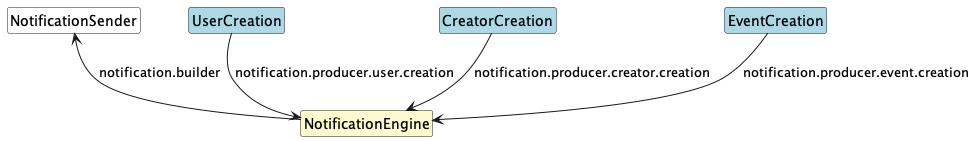
\includegraphics[width=\textwidth, height=350px, keepaspectratio]{assets/uml/structure/Creation.png}
        \end{figure}
    \end{itemize}
\end{frame}

\begin{frame}{Project Separation}
    \begin{itemize}
        \item Ticket Purchase Processes
        \begin{figure}[H]
            \centering
            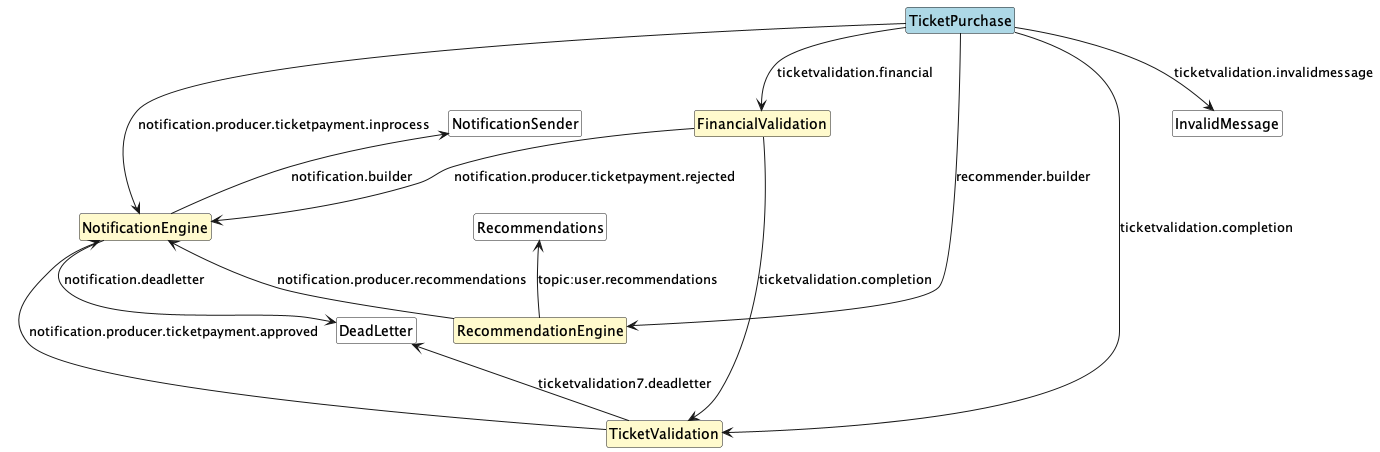
\includegraphics[width=\textwidth, height=350px, keepaspectratio]{assets/uml/structure/Purchase.png}
        \end{figure}
    \end{itemize}
\end{frame}

\section{Applications}
\begin{frame}{Applications}
    \begin{itemize}
        \item Main Application with Database connection:
        \begin{itemize}
            \item \textbf{Event Market: event-market}
        \end{itemize}
        \item Creation Camel Applications:
        \begin{itemize}
            \item \textbf{Event Creation: event-market-event-creation}
            \item \textbf{User Creation: event-market-user-creation}
            \item \textbf{Creator Creation: event-market-event-creation}
        \end{itemize}
        \item Ticket Purchase Camel Applications:
        \begin{itemize}
            \item \textbf{Ticket Purchase: event-market-ticket-purchase}
            \item \textbf{Financial Validation: event-market-financial-validation}
            \item \textbf{Ticket Validation: event-market-ticket-validation}
            \item \textbf{Event Recommender Engine: event-market-recommendation-engine}
            \item \textbf{Notification Engine: event-market-notification-engine}
        \end{itemize}
    \end{itemize}
\end{frame}

\section{Design Patterns}
\begin{frame}{Iterator and Singleton Patterns}
    \begin{itemize}
        \item \textbf{Iterator Pattern}
        \begin{itemize}
            \item Inside the \textbf{Ticket Purchase} app.
            \item Used in \textit{TicketTypeIterator} class to iterate over ticket types.
            \item Helps users browse ticket options.
        \end{itemize}
        \item \textbf{Singleton Pattern}
        \begin{itemize}
            \item Inside the \textbf{Financial Validation} app.
            \item Used in \textit{FinancialValidator} class.
            \item Ensures a single instance for validating ticket requests.
        \end{itemize}
    \end{itemize}
\end{frame}

\begin{frame}{Strategy and Facade Patterns}
    \begin{itemize}
        \item \textbf{Strategy Pattern}
        \begin{itemize}
            \item Inside the \textbf{Financial Validation} app.
            \item Used in \textit{PaymentMethod} class.
            \item Supports various payment methods like \textit{CheckingsAccountPayment} and \textit{CardPayment}.
        \end{itemize}
        \item \textbf{Facade Pattern}
        \begin{itemize}
            \item Inside the \textbf{Event Recommender Engine}.
            \item Used in \textit{EventRecommender} class.
            \item Simplifies interactions with recommendation models.
        \end{itemize}
    \end{itemize}
\end{frame}

\begin{frame}{Template Method Pattern}
    \begin{itemize}
        \item \textbf{Template Method Pattern}
        \begin{itemize}
            \item Inside the \textbf{Event Recommender Engine}.
            \item Used in \textit{AbstractRecommenderModel} and its derived classes.
            \item Provides structure for creating recommendation models.
        \end{itemize}
    \end{itemize}
\end{frame}

\section{Applications and UML Drawings}
\begin{frame}{Event Creation}
    \begin{itemize}
        \item Creates \textit{Event} instances with:
        \begin{itemize}
            \item \textit{TicketType} instances
            \item \textit{Location} instance
            \item \textit{Creator} instance
        \end{itemize}
    \end{itemize}
\end{frame}

\begin{frame}{User and Creator Creation}
    \begin{itemize}
        \item Similar to Event Creation
        \item Communicates with \textbf{Notification Engine}
    \end{itemize}
\end{frame}

\begin{frame}{Ticket Purchase}
    \begin{itemize}
        \item Handles \textit{TicketRequest} instances.
        \item Interacts with:
        \begin{itemize}
            \item \textbf{Financial Validation}
            \item \textbf{Ticket Validation}
            \item \textbf{Event Recommender Engine}
            \item \textbf{Notification Engine}
        \end{itemize}
    \end{itemize}
\end{frame}

\begin{frame}{Financial Validation}
    \begin{itemize}
        \item Validates payment for \textit{TicketRequest} instances.
        \item Uses \textit{FinancialValidator} (Singleton) and \textit{PaymentMethod} (Strategy).
    \end{itemize}
\end{frame}

\begin{frame}{Ticket Validation}
    \begin{itemize}
        \item Creates \textit{Ticket} instances from approved \textit{TicketRequest}.
        \item Updates \textit{User} with new \textit{Ticket}.
    \end{itemize}
\end{frame}

\begin{frame}{Event Recommender Engine}
    \begin{itemize}
        \item Recommends events to \textit{User} based on purchases.
        \item Uses \textit{EventRecommender} (Facade) and \textit{AbstractRecommenderModel} (Template Method).
    \end{itemize}
\end{frame}

\begin{frame}{Notification Engine}
    \begin{itemize}
        \item Translates system information into notifications.
        \item Sends messages to users and creators.
    \end{itemize}
\end{frame}

\end{document}
